\documentclass[letterpaper]{article}
\usepackage{proceed2e}
\usepackage{times}
\usepackage{helvet}
\usepackage{courier}
\usepackage{epsfig,subfigure}
\usepackage{amsmath,amsfonts,amssymb,amsthm}
\usepackage{array}
% Import some more mathematical symbols
\usepackage{amsmath,amssymb}

% Import an algorithm formatting package
\usepackage[vlined,algoruled,titlenumbered,noend]{algorithm2e}

% Define argmin, argmax
\def\argmax{\operatornamewithlimits{arg\max}}
\def\argmin{\operatornamewithlimits{arg\min}}
\def\supmax{\operatornamewithlimits{arg\sup}}

% Strikeout
%\usepackage{ulem}
%\normalem

% Define a fourth level subheading (Scott)
\newcommand{\subfour}{\vspace*{3mm}\hspace{-2mm}}
\renewcommand{\-}{\text{-}}

% Define a command for extended commenting (Scott)
\long\def\COMMENT#1\ENDCOMMENT{\message{(Commented text...)}\par}

% Define common macros
\long\def\COMMENT#1\ENDCOMMENT{\message{(Commented text...)}\par}

\newtheorem{lemma}{Lemma}[section]
\newtheorem{assumption}[lemma]{Assumption}
\newtheorem{theorem}[lemma]{Theorem}
\newtheorem{proposition}[lemma]{Proposition}
\newtheorem{corollary}[lemma]{Corollary}
\newtheorem{hypothesis}[lemma]{Hypothesis}
\newtheorem{definition}[lemma]{Definition}
%\newtheorem{hypothesis}{Hypothesis}{\bfseries}{\itshape}
%\theoremstyle{remark}
%\newtheorem*{proof_deferred}{Proof}
%\newtheorem*{proofsk}{Proof Sketch}{\rmfamily}{\rmfamily}

% No brackets after {definition},{example} starts new counters 
\newtheorem{property}[lemma]{Property}
\newtheorem{example}[lemma]{Example}
\newtheorem*{example*}{Example}

\newcommand{\norm}[1]{\textrm{\normalsize $#1$}}
\newcommand{\sm}[1]{\textrm{\footnotesize $#1$}}

\newcommand{\denselist}{\itemsep 0pt\partopsep 0pt}
\newcommand{\semidenselist}{\itemsep 2pt\partopsep 2pt}

%\def\casemax{\operatornamewithlimits{case\,max}}
\def\argmax{\operatornamewithlimits{arg\,max}}
\def\argmin{\operatornamewithlimits{arg\,min}}

%\def\argmax{\mathop{\rm arg\,max}}

%\numberwithin{algorithm}{chapter}
\newcommand{\MarsRover}{\textsc{Mars Rover}}
\newcommand{\MarsRoverL}{\textsc{Mars Rover Linear}}
\newcommand{\MarsRoverNL}{\textsc{Mars Rover Nonlinear}}
\newcommand{\InventoryControl}{\textsc{Inventory Control}}
\newcommand{\WaterReservoir}{\textsc{Water Reservoir}}
\newcommand{\MultiWaterReservoir}{\textsc{Multi-Reservoir}}
\newcommand{\Knapsack}{\textsc{Knapsack}}


\newcommand{\casemax}{\textrm{casemax}}
\renewcommand{\S}{\mathcal{S}}
\newcommand{\A}{\mathcal{A}}
\newcommand{\N}{\mathcal{N}}
\newcommand{\T}{\mathcal{T}}
\newcommand{\R}{\mathcal{R}}
\renewcommand{\L}{\mathcal{L}}
\newcommand{\I}{\mathbb{I}}
\newcommand{\F}{\mathcal{F}}
\newcommand{\G}{\mathcal{G}}
\newcommand{\X}{\mathcal{X}}
\newcommand{\op}{\;\mathit{op}\;}

\newcommand{\D}{\mathcal{D}}
\newcommand{\II}{\mathcal{I}}
\newcommand{\Gain}{\mathit{Gain}}
\newcommand{\VPI}{\mathit{VPI}}

\renewcommand{\l}{\langle}
\renewcommand{\r}{\rangle}

\newcommand{\Par}{\mathit{Par}}
\newcommand{\var}{\mathit{var}}
\newcommand{\Progress}{\mathit{Progress}}
\newcommand{\SDP}{\mathit{SDP}}
\newcommand{\BasisGen}{\mathit{BasisGen}}
\newcommand{\FOMax}{\mathit{FOMax}}
\newcommand{\EvalPolicy}{\mathit{EvalPolicy}}
\newcommand{\GetNormCacheKey}{\mathit{GetNormCacheKey}}
\newcommand{\ComputeResult}{\mathit{ComputeResult}}
\newcommand{\ModifyResult}{\mathit{ModifyResult}}
\newcommand{\GetNode}{\mathit{GetNode}}
\newcommand{\GetGNode}{\mathit{GetGNode}}
\newcommand{\Apply}{\mathit{Apply}}
\newcommand{\Reduce}{\mathit{Reduce}}

\newcommand{\BE}{\beta}
\newcommand{\AADD}{\mathit{AADD}}
\newcommand{\ADD}{\mathit{ADD}}
\newcommand{\TW}{\mathit{TW}}
\newcommand{\gre}{\mathit{gre}}
\newcommand{\Volatile}{\mathit{Volatile}}
\newcommand{\range}{\mathit{range}}

\newcommand{\Comp}{\mathit{Comp}}
\newcommand{\Sort}{\mathit{Sort}}
\newcommand{\Class}{\mathit{Class}}
\newcommand{\TBox}{\mathit{Box}}
\newcommand{\Truck}{\mathit{Truck}}
\newcommand{\City}{\mathit{City}}
\newcommand{\Plane}{\mathit{Plane}}
\newcommand{\truck}{\mathit{truck}}
\newcommand{\plane}{\mathit{plane}}
\newcommand{\tbox}{\mathit{box}}
\newcommand{\load}{\mathit{load}}
\newcommand{\loadS}{\mathit{loadS}}
\newcommand{\loadF}{\mathit{loadF}}
\newcommand{\catchFire}{\mathit{catchFire}}
\newcommand{\unload}{\mathit{unload}}
\newcommand{\unloadS}{\mathit{unloadS}}
\newcommand{\unloadF}{\mathit{unloadF}}
\newcommand{\drive}{\mathit{drive}}
\newcommand{\driveS}{\mathit{driveS}}
\newcommand{\driveF}{\mathit{driveF}}
\newcommand{\noop}{\mathit{noop}}
\newcommand{\true}{\mathit{true}}
\newcommand{\false}{\mathit{false}}
\newcommand{\BIn}{\mathit{BoxIn}}
\newcommand{\TIn}{\mathit{TruckIn}}
\newcommand{\PIn}{\mathit{PlaneIn}}
\newcommand{\On}{\mathit{BoxOn}}
\newcommand{\OnT}{\mathit{BoxOnTruck}}
\newcommand{\OnP}{\mathit{BoxOnPlane}}

\newcommand{\Road}{\mathit{Road}}
\newcommand{\Conn}{\mathit{Conn}}
\newcommand{\Rain}{\mathit{Rain}}
\newcommand{\TypeA}{\mathit{TypeA}}
\newcommand{\Up}{\mathit{Up}}
\newcommand{\reboot}{\mathit{reboot}}
\newcommand{\catchFireF}{\mathit{catchFireF}}
\newcommand{\catchFireS}{\mathit{catchFireS}}
\newcommand{\upS}{\mathit{rebootS}}
\newcommand{\upF}{\mathit{rebootF}}
\newcommand{\dropS}{\mathit{dropS}}
\newcommand{\dropF}{\mathit{dropF}}
\newcommand{\Regr}{\mathit{Regr}}
\newcommand{\DTR}{\mathit{DTR}}
\newcommand{\FODTR}{\mathit{FODTR}}
\newcommand{\scdo}{\mathit{do}}
\renewcommand{\next}{\mathit{next}}
\newcommand{\case}{\mathit{case}}
\newcommand{\aCase}{\mathit{aCase}}
\newcommand{\vCase}{\mathit{vCase}}
\newcommand{\eCase}{\mathit{eCase}}
\newcommand{\bCase}{\mathit{bCase}}
\newcommand{\pCase}{\mathit{pCase}}
\newcommand{\qCase}{\mathit{qCase}}
\newcommand{\rCase}{\mathit{rCase}}
\newcommand{\piCase}{\pi\mathit{Case}}
\newcommand{\Lif}{\mathit{if}\;}
\newcommand{\Lelse}{\;\mathit{else}\;}
\newcommand{\when}{\mathit{when}\;}
\newcommand{\then}{\;\mathit{then}\;}

\newcommand{\TAt}{\mathit{TAt}}
\newcommand{\BAt}{\mathit{BAt}}
\newcommand{\Dst}{\mathit{Dst}}
\newcommand{\paris}{\mathit{paris}}
\newcommand{\brussels}{\mathit{brussels}}
\newcommand{\moscow}{\mathit{moscow}}
\newcommand{\berlin}{\mathit{berlin}}
\newcommand{\rome}{\mathit{rome}}
\newcommand{\snow}{\mathit{snow}}

\newcommand{\mydo}{\textit{do}}
\newcommand{\open}{\textit{open}}
\newcommand{\openS}{\textit{openS}}
\newcommand{\openF}{\textit{openF}}
\newcommand{\down}{\textit{down}}
\newcommand{\downS}{\textit{downS}}
\newcommand{\downF}{\textit{downF}}
\newcommand{\up}{\textit{up}}
\newcommand{\myabove}{\textit{above}}
\newcommand{\below}{\textit{below}}
\newcommand{\EAt}{\textit{EAt}}
\newcommand{\PAt}{\textit{PAt}}
\newcommand{\OnE}{\textit{OnE}}
\newcommand{\Group}{\textit{Group}}
\newcommand{\VIP}{\textit{VIP}}
\newcommand{\Attended}{\textit{Attended}}

% Macro for strikeout text
\newlength{\howlong}
\newcommand{\sout}[1]{
\settowidth{\howlong}{#1}%
#1\unitlength0.5ex%
\begin{picture}(0,0)
\put(0,1){\line(-1,0){\howlong\divide\unitlength}}
\end{picture}%
}





\begin{document}
% The file aaai.sty is the style file for AAAI Press 
% proceedings, working notes, and technical reports.
%
\title{Symbolic Dynamic Programming for Continuous action MDPs}

%\author{Anonymous}
\author{Zahra Zamani\\
NICTA \& the ANU\\
Canberra, Australia\\
{\tt zahra.zamani@anu.edu.au}
\And
Scott Sanner\\
NICTA \& the ANU\\
Canberra, Australia\\
{\tt ssanner@nicta.com.au}
\And
?\\
?\\
{\tt ?}
}
\maketitle

\begin{abstract}
Many real-world decision-theoretic problems require continuous actions as well as continuous states in order to plan optimally. While previous works have used methods such as  discretization or approximation techniques such as sampling for the states and actions, no exact solution has been introduced for both continuous state and action spaces. In this work, we take a symbolic approach to modelling domain problems with discrete and continuous state and action Markov decision processes and propose a Dynamic programming solution to obtain the optimal policy. Our algorithm is built on symbolic manipulation such as the maximization operator and also takes into account mathematics definitions of the natural bounds on continuous action spaces. The efficient representation of Extended Algebric Decision Diagrams(XADDs) allows us to scale this algorithm for multi-variate and non-linear action spaces. We demonstrate empirical results for continuous state and action MDPs on various problems to show the first exact optimal solution to arbitrary value functions.
\end{abstract}


\section{Introduction}

\label{sec:intro}

Markov decision processes (MDPs)[2] have been a theoretical model for many planning problems in the recent years. Although the most common solution to MDPs is to use value iteration or policy iteration, they can quickly fall into Bellman's curse of dimensionality problem for large state – action spaces. In many problems this can be avoided by modelling the problem with continuous state – action spaces which is also a closer resemblance to real-world problems. \\
Examples of problems in the continuous state and action domain can include Robotics, Operation Research and Management problems. The OR (Operation Research) literature has used MDPs to model many problems such as Inventory Control [] or Water Reservoir management []. These are examples where the state space can be modelled by discrete and continuous Markov decision processes and where the actions can also be considered continuous. Most existing solutions concentrate on approximation techniques such as sampling [] that requires computational effort while providing no guarantee to the optimal solution, or other methods such as discretizing the state-action space[] that has scalability problems for large domain sizes. Meanwhile little effort has been devoted to exact solutions using the continuous variables beyond the piecewise rectilinear value function setting which contributes to a small subset of the problems in this domain. 
In the previous paper [], the solution to continuous state MDPs was investigated, here we introduce a new model for Discrete and continuous state and Action MDPs (DCA-MDPs) and propose a new algorithm for Symbolic Dynamic Programming. Although the exact solution presented in [] covers the discrete and continuous state domain, it could not be used for planning in continuous action spaces. We exploit the algebraic properties of the maximization operator for continuous actions and develop disjoint case partitions that can be used to factor the actions in the Q-value to obtain the next value function. This symbolic maximization approach allows us to go beyond the linear function domain and apply the technique for non-linear reward and transition functions. Our method is scalable to higher horizons as well as being applicable to multi-variate continuous action domains. We represent the reward function as the function that is used to reward and penalize the agent regarding its action costs. Both the reward and the transition function are represented using First-order logic with arbitrary piecewise symbol functions. These will be explained more deeply in section 2. 
The practical implementation of case statements of section 2 is the extended ADDs (XADDs) structure discussed in section 3. In section 4 the symbolic value iteration algorithm for continuous action selection is presented and the approach of maximizing the action variables is examined. Empirical results on OR problems are then demonstrated in section 5. We conclude in section 6 with a discussion on the future work. 


\section{Case Representation}

To work in the symbolic space with lifted solutions, we need a representation for the symbolic functions and logical operators. Here we define such a notation along with the required operations for the SDP algorithm in the next sections. We consider the following simple example that is used throughout this paper:

[\InventoryControl] Business firms often deal with the problem of deciding  the amount of product to order in a time period such that customer demands are satisfied. 
The firm's warehouse will keep an inventory of this product to deal with different customer demand levels. Each month, the firm must decide on the amount of products 
to order based on the current stock level. \\
The order should not be too high since keeping the inventory is expensive, nor should it be too low in which case
it will be penalized for being unable to meet customer demands and leading to loss of customers. The optimization problem faced by the firm is to find an optimal 
order policy that maximizes the profit. Inventory control has become a benchmark problem for optimization in the OR literature and applies to our general domain settings. Here we present a simple formulation of this problem: 
\vspace{+5mm}
\begin{example*}[\InventoryControl]
We consider order decisions and delivery at the beginning of each month and order satisfaction to take place at the end of the month. 
The capacity of the inventory is C units of the product and customer orders not satisfied in this month are backlogged for the next month, so inventory can take negative values.  
\\Here we have a continuous state variable $x \in [-1000,C]$ indicating the current inventory quantity, with C=500, and a stochastic boolean state variable for customer demand level $d$ where $d=0$ is low demand levels (50) and $d=1$ is high demand levels (150) according to some probability. \\
The continuous action variable is the order quantity $a \in [0,C]$ which can at most take the value of the maximum inventory capacity. \\
\end{example*}

The \textit{case} notation can present any symbolic function in the following format: 

{%\footnotesize 
\begin{align*}
f = 
\begin{cases}
  \phi_1: & f_1 \\ 
 \vdots&\vdots\\ 
  \phi_k: & f_k \\ 
\end{cases}
\end{align*}
}
Where the $\phi_i$ are logical formulaes defined over the state and action space $(\vec{d},\vec{x},\vec{a})$ that can include arbitrary logical ($\land,\lor,\neg$) combinations of the boolean variable $\vec{d}$ and can also contain any sort of
inequalities (such as $\geq,>,\leq,<$) where the left and right operands can be \emph{any} function of the continuous variables $\vec{x},\vec{a}$. 
The $f_i$ can be \emph{any} functions of the state action variables.  
\\
Each of the case statements introduce a partitioning on the domain where each partition is mutually exclusive and disjoint from the other partitions since otherwise they can be converted into more partitions with this property using logical operators: 
{%\footnotesize 
\[
\begin{cases}
\begin{array}{c}
\varphi_{1}:f_{1}\\
\varphi_{2}:f_{2}
\end{array} & \simeq\begin{cases}
\begin{array}{c}
\varphi_{1}\wedge\varphi_{2}:mutal\\
\varphi_{1}\wedge\neg\varphi_{2}\\
\neg\varphi_{1}\wedge\varphi_{2}\\
\neg\varphi_{1}\wedge\neg\varphi_{2}:nondisjoint
\end{array}\end{cases}\end{cases}
\]
}
The reward and transition functions from \InventoryControl can show the case statements in more details:
\begin{example*}
We define an immediate negative reward for the cost of producing an order ( half of the order value ) and the storage cost of holding the products in the inventory (one tenth of the total inventory stock) and also a positive reward for fulfilling the customer demand whenever there are enough stocks in the inventory.\\
We can formalize the transition and reward for \InventoryControl\ the order action using conditional equations, where $(x,d)$
and $(x',d')$ are respectively the pre- and post-action state and $R$ is immediate reward:
%\ because of backlogging, the customer demand is always taken from the current stock level, leaving it negative
%\ consider the next state as the current state and orders minus the customer orders
%\ customer demands are boolean of low and high that change in every iteration
%\ 
{\footnotesize
\begin{align*}
x' & = \begin{cases}
d     : & x + a - 150 \\
\neg d: & x + a - 50    \\
\end{cases}\\
d' & =  \begin{cases}
d     : &(0.7)\\
\neg d: &(0.3)\\
\end{cases}\\
R & = \begin{cases}
x \geq 150 \wedge d: & 150 - 0.5\cdot a - 0.1\cdot x \\
x \geq 50 \wedge \neg d: & 50 - 0.5\cdot a - 0.1\cdot x  \\
x \leq 150 \wedge d: &  (150-x)-0.5\cdot a - 0.1\cdot x \\
x \leq 150 \wedge \neg d: & (50-x)- 0.5\cdot a - 0.1\cdot x \\
\end{cases}
\end{align*}}
\end{example*}

Having defined the function notation in case statements, we now consider applying logical operators on a function. 
If the operator is \textit{Unary} such as scalar multiplications (e.g. $0.5 \cdot a$) or negation $-f$ it is simply applied to each of the disjoint partitions. 
\\ For \textit{Binary} operations, the cross-product of the logical partitions is considered and then the operator is applied to the result. The reward function is an 
example for binary $\oplus$ where the logical AND ($\wedge$) of two logical formulas  $x \geq 150 $ and $d$ is taken along with their negation, to form 4 partitions with different function definitions. \\

Likewise, $\ominus$ and $\otimes$ are applied by subtracting or multiplying partition values respectively.  
Apart from the logical operators, we also need to perform other operations such as restriction, substitution and maximization on case statements to be able to completely explain the SDP algorithm. \\

In \emph{restriction} a function $Q$ is restricted to cases that satisfy some formula $\phi$ (e.g. the binary variable $d_i$ then function can be restricted to either the true or false branch $Q|_{d_i}$).  
Restriction can be performed by appending  the logical formula (either $d_i=0 or d_i=1$) to each case partition:
{\footnotesize
\begin{center}
\begin{tabular}{r c c l}
&
\hspace{-6mm} 
  $Q = \begin{cases}
    \phi_1: & f_1 \\ 
   \vdots&\vdots\\ 
    \phi_k: & f_k \\ 
  \end{cases}$
&

&
\hspace{-2mm}
  $Q|_{d_i = 0} = \begin{cases}
    \phi_1 \land \neg d_i : & Q_1 \\ 
   \vdots&\vdots \\ 
    \phi_k \land \neg d_i : & Q_k \\ 
  \end{cases}$
\end{tabular}
\end{center}
}
%This operator will be used in computing the values of the binary demands in the next sections.\\
\emph{Symbolic substitution} takes a set $\sigma$ of variables and their substitutions, e.g., 
$\sigma = \{ d_1 / d_1', \ldots, d_n / d_n', x_1 / x_1', \ldots, x_m / x_m' \}$ where
the LHS of the $/$ represents the substitution variable and the RHS of the $/$ represents 
the expression that should be substituted in its place.\\
While the example substitutes the next state (primed) with the current state, we can use substitution again on the transition functions of the variables to build the next state completely:
 $\sigma = \{ d'/(d:0.7,\neg d:0.3), x'/(d: x + a - 150; \neg d: x + a - 50) \}$
\\For each partition, we perform substitution on the logical part $\phi$ and the functional part $f$. For the logical part of case partitions substitution occurs by applying $\sigma$ to each inequality operand. For example if $\phi_i: d' \wedge x'>200$ after substituting the result is $\phi_i\sigma : d \wedge x + a > 350 $ where with d was chosen with probability 0.7. 
\\As for the function values, they are again substituted in a similar fashion; if $f_i = 2x'+x'^{2}$ then $f_i\sigma = x^{2} + a^{2} + 2ax - 298x -298a +1950 $. The partitions remain mutually exclusive and disjoint after the substitution due to logical consequence of applying $\sigma$. Substitution is defined generally in the following:
%is this required? 
{\footnotesize
\begin{center}
\begin{tabular}{r c c l}
&
\hspace{-6mm} 
  $f = \begin{cases}
    \phi_1: & f_1 \\ 
   \vdots&\vdots \\ 
    \phi_k: & f_k \\ 
  \end{cases}$
&

&
\hspace{-2mm}
  $f\sigma = \begin{cases}
    \phi_1\sigma: & f_1\sigma \\ 
   \vdots&\vdots \\ 
    \phi_k\sigma: & f_k\sigma \\ 
  \end{cases}$
\end{tabular}
\end{center}
}
\normalsize

\emph{Symbolic maximization} is defined by considering all combinations of the logical formulas $\phi_i$ and $\psi_i$ and taking the maximum according to the function values $f$ and $g$:
\vspace{-5mm}

{\footnotesize
\begin{center}
\begin{tabular}{r c c c l}
&
\hspace{-9mm} $\max \Bigg(
  \begin{cases}
    \phi_1: & f_1 \\ 
    \phi_2: & f_2 \\ 
  \end{cases}$
$,$
&
\hspace{-4mm}
  $\begin{cases}
    \psi_1: & g_1 \\ 
    \psi_2: & g_2 \\ 
  \end{cases} \Bigg)$
&
\hspace{-4mm} 
$ = $
&
\hspace{-4mm}
  $\begin{cases}
  \phi_1 \wedge \psi_1 \wedge f_1 > g_1    : & f_1 \\ 
  \phi_1 \wedge \psi_1 \wedge f_1 \leq g_1 : & g_1 \\ 
  \phi_1 \wedge \psi_2 \wedge f_1 > g_2    : & f_1 \\ 
  \phi_1 \wedge \psi_2 \wedge f_1 \leq g_2 : & g_2 \\ 
  \phi_2 \wedge \psi_1 \wedge f_2 > g_1    : & f_2 \\ 
  \phi_2 \wedge \psi_1 \wedge f_2 \leq g_1 : & g_1 \\ 
  \phi_2 \wedge \psi_2 \wedge f_2 > g_2    : & f_2 \\ 
  \phi_2 \wedge \psi_2 \wedge f_2 \leq g_2 : & g_2 \\ 
  \end{cases}$
\end{tabular}
\end{center}
}

According to this definition, maximization of any finite number of functions can be performed by taking a pair of the functions and iteratively building the resulting maximization. For the finite number of discrete actions the following maximization results in the value function: 
\begin{align*}
V & = 
\max(Q_{a_1},\max(\ldots,\max(Q_{a_{p-1}},Q_{a_p})))
\end{align*}
Apart from this maximization, we also have to consider maximizing a function (such as the Q-function) for an infinite number of actions ($\delta$) in our continuous case. 
We present the following mathematical definitions to justify this maximization:\\

1- A real-valued function f defined on the real domain is said to have a global (or absolute) maximum point at the point x, if for all x :$ f(x^{*}) \geq f(x) $. The value of the function at this point is called maximum of the function.\\
2- Boundedness theorem states that a continuous function f in the closed interval (a,b) is bounded on that interval. That is, there exist real numbers m and M such that:
\begin{align*}
\forall x \in \{a,b\} : m \leq f(x) \leq M 
\end{align*}
3- The first partial derivatives as to x (the variable to be maximized) are zero at the maximum. The second partial derivatives are negative. These are only necessary, not sufficient, conditions for a maximum because of the possibility of saddle points.\\
Based on these definitions, the maximum value of a function is defined at the boundaries and roots of that function. If this function were linear and a polynomial of a certain degree k, then the maximum for that function would occur on any of the (k-1) roots of the function or at the lower and upper bounds defined for it. 
\\This allows us to define a maximum on a function with respect to a continuous action $\delta$, using the upper and lower bounds on each continuous action as well as the function roots. A lower bound on action $\delta$ occurs when the inequalities of $\geq ,>$ have action $\delta$ on their LHS; then any expression on the RHS is considered a lower bound on action $\delta$. Similar to this, an upper bound occurs for inequalities of $\leq , <$ and the RHS expression is considered an upper bound for action $\delta$. An example of a continuous maximization is provided below:

\vspace{-5mm}

{\footnotesize
\begin{center}
\begin{tabular}{r c c c l}
&
\hspace{-9mm} $\max \Bigg(
  \begin{cases}
\delta  \geq 0 \wedge x \leq 20: & 99-\delta \\ 
\delta \leq 200 \wedge x \geq 10: & - \delta^{2} +9 \\ 
  \end{cases}$
\end{tabular}
\end{center}
}
In this example, the lower bound of 0 and an upper bound of 200 is defined for $\delta$, as well as the maximum points of ${3,-3}$. 

\section{Extended ADDs (XADDs)}

In practice, a case statement representation of a value function with explicit
partitions is computationally expensive.  
Extended Algebric decision diagrams (XADDs) where introduced in [] and will be used 
as the development tool throughout this work. XADDs were motivated by the SPUDD~\cite{spudd} algorithm which
maintains compact value function representations for finite discrete
factored MDPs using algebraic decision diagrams (ADDs)~\cite{bahar93add},
and was extended to handle continuous variables.  An example XADD for the optimal
\InventoryControl value function is provided
in Figures1~\ref{fig:inv_v1}.
%%%%%%%%%%%%%%%%%%%%%%%%%%%%%%%%%%%%%%%%%%%%%%%%%%%%%%%%%%%%%%%%%%%%%%%%%%
\begin{figure}[t]
\begin{center}
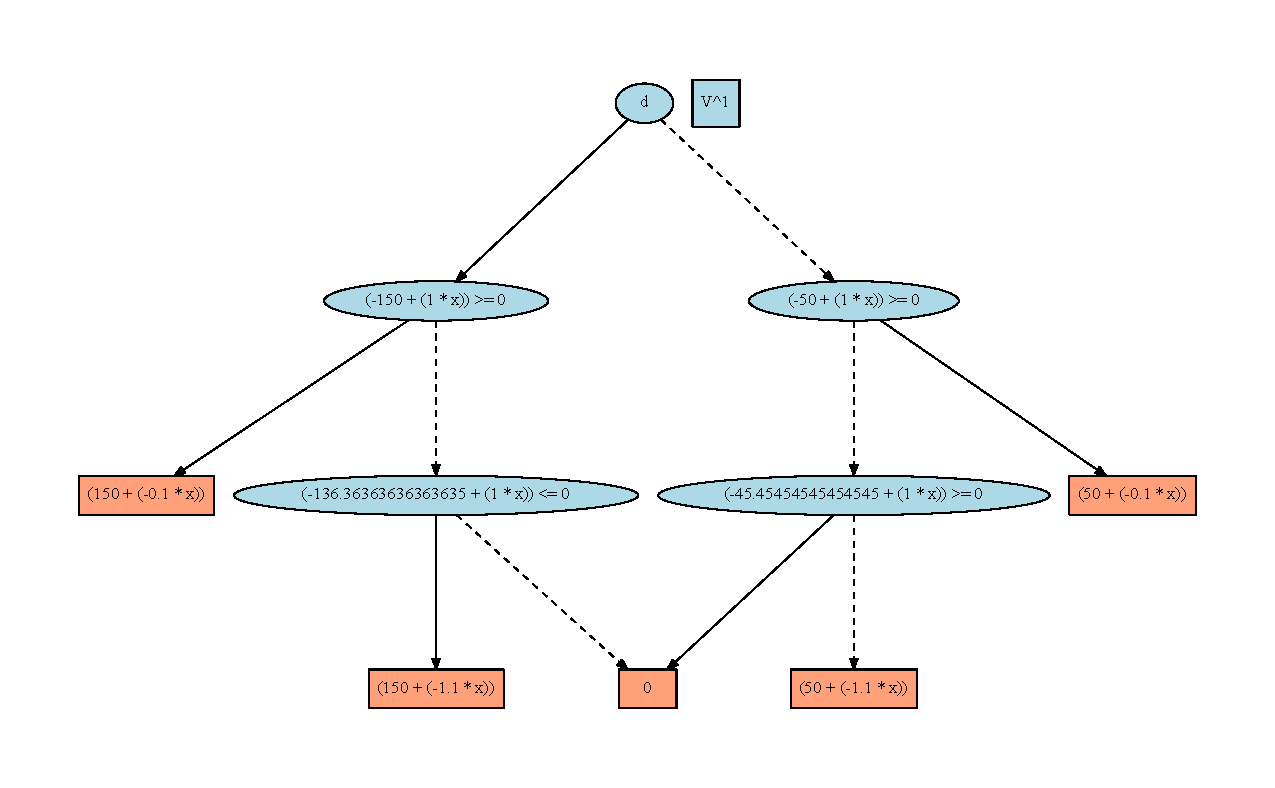
\includegraphics[width=0.4\textwidth]{Figures1/inv1.pdf}
\end{center}
\vspace{-3mm}
\caption{%\footnotesize 
The optimal value function for horizon one of \InventoryControl\ 
as a decision diagram: 
the \emph{true} branch is solid, the \emph{false}
branch is dashed.} \label{fig:inv_v1}
\vspace{-3mm}
\end{figure}
%%%%%%%%%%%%%%%%%%%%%%%%%%%%%%%%%%%%%%%%%%%%%%%%%%%%%%%%%%%%%%%%%%%%%%%%%%

In an XADD the decision nodes can have arbitrary inequalities (one
per node) and the leaf nodes can represent arbitrary functions.
Standard ADD operations to build a canonical ADD and 
to perform a binary operation on two ADDs applies in the case of XADDs.
\\
While exact solutions using symbolic dynamic
programming are possible in principle for arbitrary symbolic transition
and reward functions, we note that it is much more difficult to
devise a canonical and compact form for representations 
We will therefore restrict XADDs to use \emph{polynomial} functions only.  We note the main advantage
of this for the XADD is that we can put the leaf and decision nodes
in a \emph{unique, canonical} form, which allows us to minimize 
redundancy in the XADD representation of a case statement.
\\
It is fairly straightforward for XADDs to support all case operations defined in the previous section. 
Binary operations or restriction is done similar to the ADD case while maximization and substitution 
requires reordering of the decision nodes since the former introduces new nodes and the latter modifies
the decision nodes. 
For the maximization of continuous variables, we consider two separate XADDs for the 
upper and lower bounds on the continuous action and then apply the maximum on these two functions.\\
In general, the fact that the decision nodes have internal structure is irrelevant, but means that certain 
paths in the XADD may be inconsistent or infeasible (due to parent decisions).  To further simplify our settings, 
when the XADD has only linear decision nodes, we can use the feasibility checkers of a linear programming solver 
to prune unreachable nodes in the XADD following the approach of []. Using the XADD structure the value
iteration algorithm can scale to much longer horizons compared to the original SDP algorithm.

\section{Discrete and Continuous State-Action MDPs}

We assume that a general class of fully observable Markov decision processes with discrete and continuous states can model our domain problems.
 The state space is represented by a vector $(\vec{b},\vec{x}) = ( b_1,\ldots,b_n,x_{1},\ldots,x_m )$ consisting of Boolean variables
 $b_i$ ($1 \leq i \leq n$) such that $b_i \in \{ 0,1 \}$ and continuous Real variables $x_j$ ($1 \leq j \leq m$) s.t. $x_j \in [L_j,U_j]$ and $L_j,U_j \in
\mathbb{R}; L_j \leq U_j$.  For the action space we consider a finite number of continuous actions $A
= \{ a_1, \ldots, a_p \}$ where $a_k \in [L_k,U_k]$ and $L_k,U_k \in
\mathbb{R}; L_k \leq U_k$.
\\
The transition function is defined as the probability of the next state given the current state and action assuming the Markov property.  Considering the Dynamic Bayesian Network model for modelling each state variable and disallowing synchronic arcs in between them,  results in the following definition for the transition function:   
\begin{align}
P(\vec{b}',&\vec{x}'|\vec{b},\vec{x},a) = \label{eq:dbn} \\
& \prod_{i=1}^n P(b_i'|\vec{b},\vec{x},a) \prod_{j=1}^m P(x_j'|\vec{b},\vec{b}',\vec{x},a) \nonumber 
\end{align}

Here the first probability for binary discrete variables can be represented by conditional probability tables (CPTs). The second probability for continuous variables is represented using conditional stochastic equations (CSEs) wthat are Markovian and deterministic with the definition of any arbitrary (e.g. non-linear) function as their equation such as:
\vspace{-3mm}
{\footnotesize
\begin{align}
P(x_1' | \vec{b},\vec{b}',\vec{x},a) = \delta\left[ x_1' - 
\begin{cases}
b_1' \land x_2^2 \leq 1 : & \exp(x_1^2 - x_2^2) \\
\neg b_1' \lor  x_2^2 > 1 : & x_1 + x_2 \\
\end{cases}
\right] \label{eq:ex_csde}
\end{align}}
Using the Dirac function the conditional probability is guaranteed to integrate to 1 over the variable, furthermore the probability is stochastic since it conditions on Boolean random variables as well as sampling them stochastically at the same time. \\
The reward function represents the immediate reward of taking an action in a state and it can take the form of any arbitrary function such as:
\begin{align}
R_a(\vec{b},\vec{x}) = \begin{cases}
x_1^2 + x_2^2 \leq 1 : & 1 - x_1^2 - x_2^2  \\
x_1^2 + x_2^2 > 1 : & 0 \\
\end{cases} \label{eq:simple_reward}
\end{align}
The policy $\pi$ specifies which action to take in the current state  $(\vec{b},\vec{x})$ and the goal is to find an optimal sequence of policies
$\Pi^* = (\pi^{*,1},\ldots,\pi^{*,H})$ that maximizes the expected sum of discounted reward over a horizon $h \in H $: \\

\begin{align}
V^{\Pi^*}(\vec{x}) & = E_{\Pi^*} \left[ \sum_{h=0}^{H} \gamma^h \cdot r^h \Big| \vec{b}_0,\vec{x}_0 \right], \label{eq:vfun_def}
\end{align}
where $\gamma$ is the discount factor between 0 and 1, and  $r^h$ is the reward in horizon $h$ assuming the state state is at $h=0$.\\
This optimal policy can be obtained using the value iteration algorithm. Starting  with an initial value function, the value of taking an action in the current state is defined using the Q-function:  

\vspace{-3mm}

{\footnotesize
\begin{align}
& Q_a^{h+1}(\vec{b},\vec{x}) = R_a(\vec{b},\vec{x}) + \gamma \cdot \label{eq:qfun} \\ 
& \sum_{\vec{b}'} \int_{\vec{x}'} \left( \prod_{i=1}^n P(b_i'|\vec{b},\vec{x},a) \prod_{j=1}^m P(x_j'|\vec{b},\vec{b}',\vec{x},a) \right) V^h(\vec{b}',\vec{x}') d\vec{x}' \nonumber
\end{align}}

Now given the Q-function for each action, the h+1-stage-to-go value function is defined as: 
\begin{align}
V^{h+1}(\vec{b},\vec{x}) & = \max_{a \in A} \left\{ Q^{h+1}_a(\vec{b},\vec{x}) \right\} \label{eq:vfun}
\end{align}

If the horizon is finite then the optimal value function continues to the last horizon but if the problem has infinite horizon then a termination criteria is defined, in most problems if the value function of two successive iterations are equal, the algorithm terminates. In the next section we define the symbolic dynamic programming algorithm as the solution to DCA-MDPs.

\section{Symbolic Dynamic Programming (SDP)}

In this section we present our exact algorithm for obtaining the optimal policy for continuous action and states. This algorithm avoids approximating as well as enumerating the state and action. The Continuous state-action dynamic programming (CSA-DP) algorithm, shown in Figure ?, implements value iteration for DCA-MDPs producing a sequence of value functions $V^0,V^1,...$ until convergence and uses the XADD structure to efficiently represent state-action partitions. . \\


%%%%%%%%%%%%%%%%%%%%%%%%%%%%%%%%%%%%%%%%%%%%%%%%%%%%%%%%%%%%%%%%%
\incmargin{1em}
%\linesnumbered
\begin{algorithm}[t!]
\SetKwFunction{getCanonicalNode}{{\sc GetCanonicalNode}}
\SetKwFunction{reduce}{{\sc Reorder}}

%\SetKwInOut{Input}{input}
%\SetKwInOut{Output}{output}

%\Input{$F$ (DCA-MDP: discrete-continuous states, continuous actions, transition and reward function)}
%\Output{$F_r$ (Value function $V^h$ and optimal policy $\pi^*$)}
\BlankLine
\Begin{
   \textbf{if} R is action independent \textbf{then} set $V^0=R$     \textbf{else} $V^0 = 0$\\
   \While {$h < \mathit{maxHorizon}$}{
      	\ForEach { action variable a in A }{
      		Prime Value function ($V^{'h}$)using Substitution\\
      		\ForEach {continuous state variable in S}{
      			Perform Continuous integration: 
      			\[
      			\tilde{Q}_a^{h+1} :=\int_{x_j'} \delta[x_j' - g(\vec{x})] V'^{h} dx_j' \; = \; V'^{h} \{x_j' / g(\vec{x}) \}
      			\]
      		}\\
      		\ForEach {discrete state variable in S }{
      			Perform Discrete marginalization: 
      			\[
      			\tilde Q_a^{h+1} := \left[\tilde Q_a^{h+1} \otimes P(b_i'|\vec{b},\vec{x},a) \right]|_{b_i' = 1} \nonumber 
      		   	 \oplus \left[\tilde Q_a^{h+1} \otimes P(b_i'|\vec{b},\vec{x},a) \right]|_{b_i' = 0}
      		    \]
      		}
      		\\
      		
      		
      	}
      }
}
\caption{{\sc CSA-DP} }
\end{algorithm}
\decmargin{1em}
%%%%%%%%%%%%%%%%%%%%%%%%%%%%%%%%%%%%%%%%%%%%%%%%%%%%%%%%%%%%%%%%%
We now describe each section of the algorithm with our \InventoryControl example. 
\begin{enumerate}
\item The symbolic value iteration algorithm works with the XADD structure for efficiency. This means that each of the i-stage-to-go value functions ($V^i$) is set to be an XADD. In most problems in this domain, the reward function defines action costs as a penalty to avoid the agent of acting more than required. For this reason we define the first value function equal to zero $V^0=0$ which is a tree with only one leaf node [0]. If the reward function of the DCA-MDP is independent of the actions, then the first value function can be equal to this reward $V^0=R$.\\

\item Next, for $h > 0$ the algorithm iterates over the horizon until a convergence criteria is met or in our case the maximum number of iterations is reached. The next parts of the algorithm is performed for each horizon. For each horizon we take each action (can be discrete or continuous) and perform the following steps in sequence.\\

\item The first step of value iteration for horizon h, action a is to prime the current state so it becomes the next state. This can be performed by substituting the state variables with their primed versions. Given as an example in section 2, we set
$\sigma = \{ d_1 / d_1', \ldots, d_n / d_n', x_1 / x_1', \ldots, x_m / x_m' \}$
and obtain $V'^{h} = V^{h}\sigma$.

\item Next, we need to consider the back-up step of the Bellman equation of ~\eqref{eq:qfun} restated here: 
 \vspace{-3mm}
 
 {\footnotesize
 \begin{align}
 & Q_a^{h+1}(\vec{b},\vec{x}) = R_a(\vec{b},\vec{x}) + \gamma \cdot \label{eq:qfun} \\ 
 & \sum_{\vec{b}'} \int_{\vec{x}'} \left( \prod_{i=1}^n P(b_i'|\vec{b},\vec{x},a) \prod_{j=1}^m P(x_j'|\vec{b},\vec{b}',\vec{x},a) \right) V^h(\vec{b}',\vec{x}') d\vec{x}' \nonumber
 \end{align}}
 
We first evaluate the integral marginalization $\int_{\vec{x}'}$ over the continuous variables in the algorithm. For each of the continuous variables $x'_j$, the only functions dependent on this variable are $V'^{h}$
and $P(x_j'|\vec{b},\vec{b}',\vec{x},a) = \delta[x_j' - g(\vec{x})]$; 
hence, marginal over $x_j'$ need only be computed over
their product. Also according to [] this integration is equal to substituting $\sigma = \{ x_j' / g(\vec{x}) \}$
on $V'^{h}$, that is
\begin{align}
\int_{x_j'} \delta[x_j' - g(\vec{x})] V'^{h} dx_j' \; = \; V'^{h} \{x_j' / g(\vec{x}) \} . \label{eq:one_int}
\end{align}

This substitution is performed for each $x_j'$ ($1 \leq j \leq m$). Stochastic   The only
additional complication is that the form of 
$P(x_j'|\vec{b},\vec{x},a)$ is a \emph{conditional} 
equation, c.f.~\eqref{eq:ex_csde}, and represented generically
as follows:
\begin{align}
   P(x_j'|\vec{b},\vec{x},a) = \delta\left[ x_j' = \begin{cases}
    \phi_1: & f_1 \\ 
   \vdots&\vdots\\ 
    \phi_k: & f_k \\ 
  \end{cases} \right] \label{eq:cond_sub}
\end{align}
Hence to perform~\eqref{eq:one_int} on this more general
representation, we obtain that $\int_{x_j'} P(x_j'|\vec{b},\vec{x},a) V'^{h} dx_j'$
\begin{align*}
    = \begin{cases}
    \phi_1: & V'^{h} \{ x_j' = f_1 \} \\ 
   \vdots&\vdots\\ 
    \phi_k: & V'^{h} \{ x_j' = f_k \}  \\ 
  \end{cases}
\end{align*}
In effect, we can read~\eqref{eq:cond_sub} as a \emph{conditional
substitution}, i.e., in each of the different \emph{previous state}
conditions $\phi_i$ ($1 \leq i \leq k$), we obtain a different
substitution for $x_j'$ appearing in $V'^{h}$ (i.e., $\sigma = \{ x_j' / f_i
\}$).  Here we note that because $V'^{h}$ is \emph{already} a case
statement, we can simply replace the single partition $\phi_i$ with the
multiple partitions of $V'^h \{ x_j' / f_i \}|_{\phi_i}$.\footnote{If $V'^h$
had mutually disjoint partitions then we note the restriction and
substitution operations preserve this disjointness.}  This reduces
the \emph{nested} case statement back down to a non-nested case
statement as in the following example:
\begin{align*}
    \begin{cases}
      \phi_1: & 
        \begin{cases}
          \psi_1: & f_{11} \\ 
          \psi_2: & f_{12}  \\ 
        \end{cases} \\
      \phi_2: & 
        \begin{cases}
          \psi_1: & f_{21} \\ 
          \psi_2: & f_{22}  \\ 
        \end{cases} \\
    \end{cases} & \; = \;
        \begin{cases}
          \phi_1 \land \psi_1: & f_{11} \\ 
          \phi_1 \land \psi_2: & f_{12}  \\ 
          \phi_2 \land \psi_1: & f_{21} \\ 
          \phi_2 \land \psi_2: & f_{22}  \\ 
        \end{cases} 
\end{align*}

To perform the full continuous integration, 
if we initialize 
$\tilde{Q}_a^{h+1} := V'^{h}$ for each action $a \in A$, and repeat
the above integrals for all $x_j'$, updating $\tilde{Q}_a^{h+1}$ each time,
then after elimination of all $x_j'$ ($1 \leq j \leq m$), we will have 
the partial regression of $V'^{h}$ for the continuous variables for
each action $a$ denoted by $\tilde{Q}_a^{h+1}$.
\item {\it Discrete Marginalization}: Now that we have our partial
regression $\tilde{Q}_a^{h+1}$ for each action $a$, we proceed
to derive the full backup $Q_a^{h+1}$ from $\tilde{Q}_a^{h+1}$
by evaluating the discrete 
marginalization $\sum_{\vec{b}'}$ in~\eqref{eq:qfun}.
Because we previously disallowed synchronic arcs
between the variables in $\vec{b}'$ 
in the transition DBN, we can sum out each variable $b_i'$ ($1 \leq i \leq n$) 
independently.  Hence, initializing
$Q_a^{h+1} := \tilde{Q}_a^{h+1}$
we perform the discrete regression by applying the following iterative
process \emph{for each} $b_i'$ in any order
for each action $a$:
\begin{align}
Q_a^{h+1} := & \left[ Q_a^{h+1} \otimes P(b_i'|\vec{b},\vec{x},a) \right]|_{b_i' = 1} \nonumber \\
 & \oplus \left[ Q_a^{h+1} \otimes P(b_i'|\vec{b},\vec{x},a) \right]|_{b_i' = 0}.
\end{align}
This requires a variant of the earlier restriction operator $|_v$ that
actually \emph{sets} the variable $v$ to the given value if present.
Note that both $Q_a^{h+1}$ and $P(b_i'|\vec{b},\vec{x},a)$ can be represented
as case statements (discrete CPTs \emph{are} case statements), 
and each operation produces a case statement.
Thus, once this process is complete, we have marginalized over
all $\vec{b}'$ and $Q_a^{h+1}$ is the symbolic representation
of the intended Q-function.
\item {\it Maximization}: Now that we have $Q_a^{h+1}$ in
case format for each action $a \in \{a_1,\ldots,a_p\}$, obtaining
$V^{h+1}$ in case format as defined in~\eqref{eq:vfun} requires
sequentially applying
\emph{symbolic maximization} as defined previously:
\begin{align*}
V^{h+1} & = 
\max(Q_{a_1}^{h+1},\max(\ldots,\max(Q_{a_{p-1}}^{h+1},Q_{a_p}^{h+1})))
\end{align*}
\end{enumerate}
By induction, because $V^0$ is a case statement and applying
SDP to $V^h$ in case statement form produces $V^{h+1}$ in case
statement form, we have achieved our intended
objective with SDP.  On the issue of correctness,
we note that each operation above simply implements one of the
dynamic programming operations in \eqref{eq:qfun} or \eqref{eq:vfun}, 
so correctness simply follows from verifying (a) that each case
operation produces the correct result and that (b) each case operation
is applied in the correct sequence as defined in \eqref{eq:qfun} or 
\eqref{eq:vfun}.  
This partial Q-value ( ) is performed for one of the continuous actions (Δ) generating an XADD with both the state and action variables at the leaf nodes and in the decisions. 
\begin{align}
V^{h+1}(\overrightarrow{b},\overrightarrow{x})=max_{a_{1},...,a_{p}}\{max_{\bigtriangleup}Q_{ad}(\bigtriangleup,x,b)\}
\end{align}
The resulting XADD of figure ?? is the input to this algorithm for solving  $\{max_{\bigtriangleup}Q_{ad}(\bigtriangleup,x,b)\}$.
According to this XADD, we can take the maximum of the entire XADD to be equal to the taking the maximum value for Δ in each of the partition values at the leaves, such that the constraints on the decision nodes hold. Symbolically this is equivalent to stating that the maximum value of an action over different case-statements is equal to taking the maximum of each of the function definitions of the case-statements separately with respect to their constraints.
//max equation of cases
The next theorem is used to evaluate the maximum value for each of the XADD partitions. 
Put theorem, if found!  
To put the above theorem in simple words, The maximum value of a function is defined at the boundaries and roots of that function in the space. If this function were linear and a polynomial of a certain degree k, then the maximum for that function would occur on any of the (k-1) roots of the function or at the lower and upper bounds defined for it. Figure ?? shows this property for a polynomial of degree ?. Mathematically this allows us to use the upper and lower bounds on each continuous action as well as the function roots to determine the optimal value function. The maximum action is then just the argmax() of this value. 
The XADD structure allows us to efficiently use the above theorem for continuous actions on the Q-function and obtain the maximum value function. The function roots is defined by taking the first derivative of each of the leaf nodes according to Δ and setting it equal to zero. The corresponding results such as the one illustrated below can be one of the maximum Q-function values. 
As for the upper and lower bounds, the decision nodes in each partition are the constraints required to define the bounds on Δ. Considering each leaf as the function to maximize, that paths to reach that leaf have to be considered separately. In each path there are a number of decision nodes. Each decision node is an inequality that either has the Δ variable in it or not. If the decision contains the variable Δ it is considered as a potential upper or lower bound for Δ. We apply the following steps in order to build the XADD: 
I.Consider two empty XADDs for the lower and upper bounds.
II.Isolate the action variable Δ one the left hand side of the inequality. This means taking terms without Δ to the other side and dividing by the coefficient of Δ. 
III.If the divisor is negative or this decision is from the false branch of the XADD, flip the inequality sign. 
IV.If the inequality is greater or greater to equal (>,>=) take the maximum over the right hand side of this inequality and the current lower bound tree, the result is the maximum lower bound in an XADD.
V.Else (if <,<=) take the minimum of the right hand side of the inequality and the current upper bound XADD. 
VI.Perform this for all the decision nodes for that leaf to obtain two XADDs of the possible upper and lower bounds. 
VII.We substitute every occurrence of Δ in the leaf node with the boundaries, which are XADD trees.
VIII.We obtain the overall maximum boundary by taking the maximum of the substituted lower and upper bound XADDs. 

For the decision nodes that don’t have Δ, we consider them as irrelevant nodes that are only multiplied in the final product XADD from the previous step. This will ensure the the resulting XADD is product of considering all the constraints of this partition leading to this leaf node. Figure ?? shows the visual illustration of this process for our running example. 
This symbolic maximization can be easily extended to any arbitrary function with complicated and non trivial constraints. Figure ?? shows the resulting XADD for the example below: 

For each of the leaves in the XADD of   this algorithm is performed to obtain the maximum value for that leaf. The overall maximum of all the leaves is stored in an XADD and in each stage, a new maximum of a leaf is multiplied to the current maximum of the leaves. The resulting XADD is then pruned and the resulting Q-function Q is used as the initial point for the next continuous action variable. This process is performed for all the continuous actions in the finite set of actions, thus returning the maximum over all possible actions on   Returning the maximum of all the Q-functions for the action set is equal to the action-independent value function of equation (??). 

%To make this concrete, we provide an example of SDP for \Knapsack.

On a final note, we observe that SDP holds for \emph{any} symbolic
case statements; we have not restricted ourselves to rectangular
piecewise functions, piecewise linear functions, or even piecewise
polynomial functions.  As the SDP solution is purely symbolic,
SDP applies to \emph{any} DC-MDPs using bounded symbolic function 
that can be written in case format!  Of course, that is the theory,
next we meet practice.




\section{Empirical Results}



\subsection{Domains}

\paragraph{\WaterReservoir}The problem of \WaterReservoir needs to make an optimal decision on how much and when to discharge water from multiple water reservoirs to maximize hydroelectric energy productions while considering environment constraints such as irrigation requirements and flood prevention. This problem is often considered using 
one single reservoir since in the multiple case the outflow of upstream reservoirs affect the inflow of downstream reservoirs. Mathematical multivariate models such as autoregressive  processes using the historical mean and variance of a site is used []. 
The state is the tuple $(l,i,e)$ with the continuous variable $l_i \in\mathbb{R}$ the water level of the i-th reservoir,

A multi-reservoir system is more desirable than the single reservoir problem due to its ability in controlling various environment parameters such as flooding. 
In these systems, the inflow of downstream reservoirs are effected by the outflow of their upstream reservoirs. In the OR literature, this case 
is considered much more complex and for the sake of simplicity mainly the single case in considered. For multi-reservoirs the main problem that leads to 
approximations to DP methods or using other simplifications is the curse of dimensionality. In this domain the discharge action is considered as a discrete action 
and so are the energy demands. This causes the state space to grow exponentially in case of multiple states and actions.[]
Using our method for continuous action value iteration, we show that this problem can be handled efficiently and is scalable to multi-reservoir problems. 

\paragraph{\MultiWaterReservoir} Consider a two-level reservoir with the outflow of the second reservoir added to the input of the first reservoir. The state space is the level of water in both reservoirs as well as the energy demands and inflow (such as rainfall or streams) to the reservoirs $(l1,l2,i,e)$. We consider the water levels as continuous variables, the inflows to both reservoirs are the same which depends on a high-low sessions of rainfall. The energy demands can be considered both continuous or discrete, here we assume the customers either want high energy around 700 units(e.g. in winter or summer) or low energy of about 350 units (e.g. in spring or autumn). 
The discharge actions of both reservoirs are considered continuous $(d1,d2)$. For the transition we define the following equations: 

{\footnotesize
\begin{align*}
l1' & = \begin{cases}
i     : & l1 + 100 +d2  - d1 \\
\neg i: &  l1 + 50 +d2  - d1   \\
\end{cases}\\
l2' & =  \begin{cases}
i     : &l2+100 - d2\\
\neg i: &l2+50 - d2\\
 \end{cases}\\
 e' & = \begin{cases}
 e     : & (0.7) \\
 \neg e: &  (0.3)   \\
 \end{cases}\\
i' & = \begin{cases}
i     : & (0.7) \\
\neg i: &  (0.3)   \\
\end{cases}\\
\end{align*}}

As for the reward function, we consider a reward of the energy demand multiplied by the price per unit if the demand is fulfilled. The energy  If the demand is not reached, then only
the amount discharged will get this reward. There is also a penalty for reaching low water levels and a higher penalty for very high water levels to prevent unsatisfied customers and  flooding. The reward function can be formulized as below: 

{\footnotesize
\begin{align*}
R & = \begin{cases}
(d1+d2) \geq 700 \wedge (50 \leq 4000 \wedge 50 \leq 4000) :\\
\textit{0.3*700}  \\
(d1+d2) \geq 700 \wedge \neg (50 \leq 4000 \wedge 50 \leq 4000) :\\
\textit{0.3*700-0.5*(50-l1-l2)-0.01*(l1+l2)}  \\
(d1+d2) \leq 700 \wedge (50 \leq 4000 \wedge 50 \leq 4000): \\
\textit{0.3*(d1+d2)} \\
(d1+d2) \leq 700 \wedge \neg (50 \leq 4000 \wedge 50 \leq 4000): \\
\textit{0.3*(d1+d2)-0.5*(50-l1-l2 -0.01*(l1+l2)} \\
(d1+d2) \geq 350 \wedge (50 \leq 4000 \wedge 50 \leq 4000): \\
\textit{0.3*350} \\
(d1+d2) \geq 350 \wedge \neg (50 \leq 4000 \wedge 50 \leq 4000): \\
\textit{0.3*350-0.5*(50-l1-l2)-0.01*(l1+l2)}\\
(d1+d2) \leq 350 \wedge (50 \leq 4000 \wedge 50 \leq 4000): \\
\textit{0.3*(d1+d2)} \\
(d1+d2) \leq 350 \wedge \neg (50 \leq 4000 \wedge 50 \leq 4000): \\
\textit{0.3*(d1+d2)-0.5*(50-l1-l2)-0.01*(l1+l2)}\\
\end{cases}
\end{align*}}

According to the transition and reward function, the value iteration is performed for this problem using the algorithm explained in section 4.


\subsection{Results}



\section{Related Work}



\section{Conclusions}



\section*{Acknowledgements}



\bibliography{cont_mdp}
\bibliographystyle{plain}

\end{document} 
